\documentclass[USenglish]{article}
%3,000 and 4,000 w
\ifx\directlua\undefined\ifx\XeTeXcharclass\undefined
  %\usepackage[utf8]{inputenc}                           %pdftex engine
  \else\RequirePackage[no-math]{fontspec}[2017/03/31]\fi %xetex engine
  \else\RequirePackage[no-math]{fontspec}[2017/03/31]\fi %luatex engine
\usepackage[small]{dgruyter}


%analysis to do
% let's just do a ridgeplots


% check the degree of multivalues. UD says: "It is possible to declare that a feature has two or more values for a given word: Case=Acc,Dat. The interpretation is that the word may have one of these values but we cannot decide between them. Such multivalues should be used sparingly. They should not be used if the value list would cover the whole value space, or the subspace valid for the given language. That would mean that we cannot tell anything about this feature for the given word, and then it is preferable to just leave the feature out." 

% discuss: "Not mentioning a feature in the data implies the empty value, which means that the feature is either irrelevant for this part of speech, or its value cannot be determined for this word form due to language-specific reasons." https://universaldependencies.org/u/overview/morphology.html

% genres
% should we try subset on  Parallel Universal Dependencies (PUD) tre

% Unicode
%\usepackage[utf8]{inputenc}
\usepackage{hyperref}
\hypersetup{
	unicode,
%	colorlinks,
%	breaklinks,
%	urlcolor=cyan, 
%	linkcolor=blue, 
	pdfauthor={Author One, Author Two, Author Three},
	pdftitle={A simple article template},
	pdfsubject={A simple article template},
	pdfkeywords={article, template, simple},
	pdfproducer={LaTeX},
	pdfcreator={pdflatex}
}

\usepackage{booktabs}
\usepackage{multirow}
\usepackage{placeins}
\usepackage{natbib}
% Theorem, Lemma, etc

\usepackage{graphicx, color}
\graphicspath{{latex/fig/}}

\begin{document}

%  \articletype{...}

  \author*[1]{Hedvig Skirgård}
  \author[1]{Stephen Francis Mann}
%  \runningauthor{...}
  \affil[1]{Department of Linguistic and Cultural Evolution, Max Planck Institute for Evolutionary Anthropology, Leipzig, Germany}
%  \affil[2]{...}
  \title{Using annotated corpora to explore morphological information}
%  \runningtitle{...}
%  \subtitle{...}
  \abstract{
  The emergence of annotated corpora collections in many different languages opens up new avenues for research in linguistic typology which take into account more nuances of language use.
    In this paper, we use the morphology annotations in the Universal Dependencies datasets (UD) to quantify the information carried by morphological features.
    We propose an approach founded in information theory which focusses on how surprising a certain morphological annotation is given a token's lemma.
    This metric is sensitive to how the morphological annotations are distributed in the data.
    For example, if the tokens of certain lemma have the value IMP for ASPECT 95\% of the time and otherwise PERF, then ASPECT is less informative than if the distribution was 50/50.
    We use these proportions to calculate how surprising the morphological annotation for a given token is and use this to measure overall how much information is carried by morphology in different UD datasets.
    We find that languages vary in how much information is encoded in morphology and that the variation correlates moderately with measurements of fusion, which is a metric that has been used to quantify ``linguistic complexity''.
    We argue that measurements such as the one presented in this paper makes it possible to test more specific hypotheses of ``linguistic complexity'', such as informational load distribution of different parts of language and even non-linguistic domains.
    We also discuss possible modifications to the approach (generalising over part-of-speech or other categories instead of lemma) and shortcomings (reliability of morphological annotation, null-marking, conditional probabilities etc).  
  }
  \keywords{morphology, Universal Dependencies, corpora, information theory, surprisal}
%  \classification[PACS]{...}
%  \communicated{...}
%  \dedication{...}
%  \received{...}
%  \accepted{...}
%  \journalname{...}
%  \journalyear{...}
%  \journalvolume{..}
%  \journalissue{..}
%  \startpage{1}
%  \aop
%  \DOI{...}

\maketitle
	
\newpage
\section{Introduction}
Do some languages necessarily encode more information than others?
All languages can express all concepts, albeit in different ways and perhaps at varying length. 
There may not be a word for the German expression ``schadenfreude'' in all languages, but we can approximate the meaning (though it may take us several words - even several clauses). 
Grammar is the set of rules of a language that determine how to put units together, and what has to be specified. 
``grammar [...] determines those aspects of each experience that must be expressed'' \citep[132]{boas1938language}. 
Languages differ in their grammar, which means they also differ in what ``must be expressed''. 
For example, some languages have pronoun systems with a distinction between inclusive and exclusive ``we'' (e.g. S\={a}moan l\={a}tou / m\={a}tou). 
While the English language does not have such a grammatical distinction in its pronoun system, the information can be expressed optionally in English (e.g. ``we, you and I, are going''). 
In English, this information is optional and the utterance can be left ambiguous between including the hearer or not without being ungrammatical. In S\={a}moan, the distinction is made every time ``we'' is expressed. 
The grammar of S\={a}moan entails a higher degree of information specificity in this particular regard. There is other information that English grammar specifies which S\={a}moan does not, such as masculine / feminine gender on 3rd person pronouns.

We can compare languages in terms of how much specific information their grammars determine. In this paper we investigate this using cross-linguistic corpora, and we also study how those distinctions are used in terms of their frequency. For example, it is possible that a particular grammatical distinction exists in a language such that there are two alternatives, but 90\% of the time speakers just use one alternative. Such a distinction is less informative than one that shows more variation between the alternatives frequency.

Informational distinctiveness in grammar is one of the concepts that is covered by the term ``language complexity''. In this paper we give a brief overview of research on ``language complexity'' and where this study is situated.


\section{Background}\label{sec:background}
\subsection{Language complexity''}
%Measuring information
Language complexity has fascinated linguists and other scholars for a long time. There are many theories, primarily relating language complexity to contact languages \citep{mcwhorter_2003} and population size and/or proportion of non-native speakers (inter alia \citet{wray2007consequences, dahl2004growth, lupyan2010language, bentz2013languages, bentz2015adaptive, raviv2019larger, koplenig2019language, shcherbakova2023societies}). Broadly one can characterise the field of research as being concerned with how and under what conditions languages acquire more complexity than would seem necessary for pure information transmission and how such complexity can be lost.
Language complexity can be operationalised into different specific measurements. 
Some of these measurements are correlated \citep{bentz2016comparison}, however as they map onto different theories of causation and phenomena in the languages themselves they can be significantly different (cf. \citet{lupyan2024cautionary}). 
Table \ref{tab:complex_metrics} gives an overview of several different ways of measuring language complexity. Note that for some of the measurements, there are instantiations using typological survey of grammars or language corpora.


\begin{table}[h]
    \centering
    \begin{tabular}{p{3cm}p{3.5cm}p{2.5cm}p{2cm}p{2cm}}  % Adjust column alignment as needed
        \toprule
        \textbf{Metric} & \textbf{Description} & \textbf{Data source} & \textbf{Studies \newline(selection)} \\ 
        \midrule
       \multirow{2}{2.5cm}{boundedness/fusion}   & \multirow{2}{3.5cm}{how much grammatical material is morphologically bound to verb/noun/other Part-of-Speech (c.f. isolating/agglutinating/ synthetic) } & typological survey of grammars & \cite{grambank_release}; \cite{shcherbakova2023societies} \\ 
        \cmidrule{3-4}
         &  & language corpora \newline \\ 
         \midrule
        type-token-ratio (TTR) & how many unique words in relation to all words (more morphology = more unique words) & language corpora &  \cite{kettunen2014can}\\ 
               \midrule
     \multirow{2}{3cm}{information/ informativity}     & \multirow{2}{3.5cm}{how much information is expressed (via grammar/words)} & typological survey of grammars & \cite{shcherbakova2023societies} \\
       \cmidrule{3-4}
      &  & natural language corpora \\    \midrule
redundancy  & how much information is repeated &&  \cite{leufkens2023measuring}\\    \midrule
systematicity/ transparency  & the degree of consistency of form to meaning patterns && \cite{raviv2019larger}; \cite{hengeveld2018transparent} \\    \midrule
regularity & the consistency of rules, for example in paradigms & & \cite{round2022cognition}\\    \midrule
compositionality  & The extent to which the meaning of larger units is built from the meanings of smaller parts &  &\cite{wray2007consequences} \\    \midrule
compressibility  & how much a computer algorithm can compress language material & & \cite{juola1998measuring} \\    \midrule
ease of LLM-learning  & how easy is it for an LLM to learn the language & & \cite{koplenig2023languages}  \\    \midrule

prediction accuracy  & how accurately the next item can be predicted && \cite{frank2011insensitivity} \\    \midrule
length of syntactic dependencies  &  how nested the syntactical structure is (tax on short-term memory) && \cite{gibson1998linguistic}; \citet{liu2008dependency} \\    
\midrule
shared types & the total number of population-wide shared types & simulations only & \citet{spike2017population}\\
\bottomrule
    \end{tabular}
    \caption{Non-exhaustive table of different language complexity metrics.}
    \label{tab:complex_metrics}
\end{table}

These different measurements can be loosely associated with four broader facets of language complexity:

\begin{itemize}
\item easy of learning as a child's first language(s)
\item easy of learning as additional language when adult
\item ease of production for sender (a.k.a encoding complexity)
\item ease of processing/comprehension for receiver (a.k.a decoding complexity)
\end{itemize}

Fig \ref{fig:metrics_diagram} illustrates possible connections between the different measurements and these four larger categories.

\begin{figure}[ht]
    \centering
    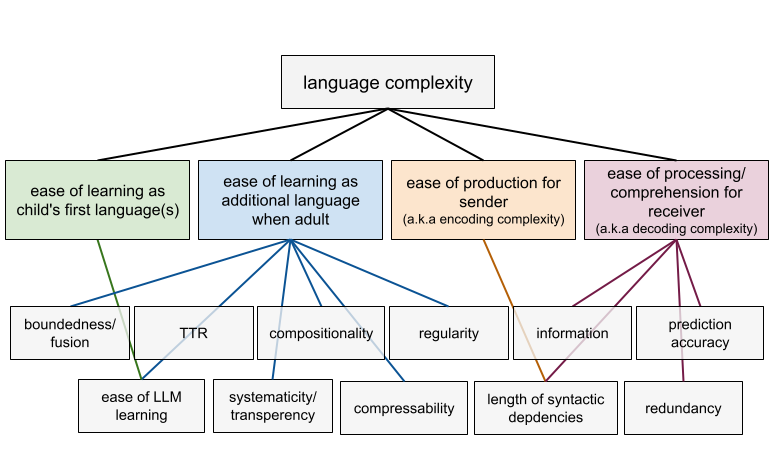
\includegraphics[width=0.9\textwidth]{latex/graphics/ud_complexity_metrics.png} % Change filename and width as needed
    \caption{Diagram of measurements of language/linguistic complexity.}
    \label{fig:metrics_diagram}
\end{figure}

In this paper, we are primarily interested in the pragmatics of information transfer between adult native speakers and how the trade-off between the encoding and decoding cost is balanced in different languages. Specifically, we are interested in variations with respect to morphological information.


%insert ackerman and malouf (2009) and Cotterell (2019) into regularity?

%Ackerman, Farrell, James P. Blevins & Robert Malouf. 2009. Parts and wholes: Implicative patterns in inflectional paradigms. In James P. Blevins & Juliette Blevins (eds.), Analogy in grammar: Form and acquisition (Oxford Linguistics), 54–82. Oxford: Oxford University Press.

%Cotterell, Ryan, Christo Kirov, Mans Hulden & Jason Eisner. 2019. On the complexity and typology of inflectional morphological systems. Transactions of the Association for Computational Linguistics 7. 327–342.


\FloatBarrier
\section{Study outline}
The aim of this study is to quantify the information in morphology annotations in corpora as a way of assessing how much information is being encoded. This can be understood as decreasing the ease of production for the sender, and thereby increasing one facet of language complexity.

Many corpora collections, such as the Universal Dependencies datasets v2.14 \citep{UD_2.14} which is used here, contain information on the morphology of individual words. Table \ref{tab:turkish_example} is an example of a sentence in Turkish where words are marked for case, number, person, aspect and more grammatical categories \citep{kuzgun_2020_UD_turkish_penn}.
For example, the word ``horses'' in English would typically be tagged for the grammatical meaning ``plural'' being encoded morphologically.
In this study, we are not only interested in how many morphological features on average a token in a given language has - but also how informative those features are given their lemma\footnote{For this paper, we focussed on the relative frequencies of morphological features given the lemma, but it's also possible to condition on part-of-speech.}. 

\begin{table}[h]
    \centering
    \caption{Sentence 15-0000 from Universal Dependencies dataset Turkish-Penn \citep{kuzgun_2020_UD_turkish_penn}. upos : Universal Part-of-Speech, lemma = base form, token = specific word, feats = morphological features} %note table captions go above the table
    \label{tab:turkish_example}   
    \begin{tabular}{p{1.5cm}p{2cm}p{2cm}p{6cm}}
\toprule
	\textbf{upos}	&	\textbf{lemma}	&	\textbf{token}	&	\textbf{feats}	\\
    \midrule
	ADJ	&	devasa	&	Devasa	&	\\    \midrule
	ADJ	&	ölçek	&	ölçekli	&\\    \midrule
ADJ	&	yeni	&	yeni	&		\\    \midrule
	NOUN	&	kanun	&	kanunda	&	Case=Loc|Number=Sing|Person=3	\\    \midrule
	ADJ	&	kullan	&	kullanılan	&		\\    \midrule
ADJ	&	karmaşık	&	karmaşık	&\\    \midrule
CCONJ	&	ve	&	ve	&		\\    \midrule
ADJ	&	çetrefil	&	çetrefilli	&		\\    \midrule
	NOUN	&	dil	&	dil	&	Case=Nom|Number=Sing|Person=3	\\    \midrule
	NOUN	&	kavga	&	kavgayı	&	Case=Acc|Number=Sing|Person=3	\\    \midrule
	VERB	&	bulan	&	bulandırdı	&	Aspect=Perf|Mood=Ind|Number=Sing| Person=3|Polarity=Pos|Tense=Past| VerbForm=Fin|Voice=Cau	\\\midrule
   \multicolumn{4}{p{11cm}}{Translation: \textit{The complex and complicated language in the massive new law has muddied the fight.}}\\    \bottomrule


    \end{tabular}
\end{table}

Words can be grouped according to their lemma (base-form). 
For example ``horse'', ``horses'', ``horse's (possessive)'' all have the same lemma, usually represented in the singular, nominative non-possessive form, i.e. ``horse''.
The information stored in the morphological feature on the token can be understood as dependent on the relative frequencies of that feature on that lemma. 

For example, in the Turkish-Penn dataset of Universal Dependencies 2.14 there are 52 tokens with the lemma ``kanun'' (Eng: \textit{law}). 47 of those tokens are marked as singular for the number category, and 5 as plural. Most of the time when people use this word in this corpus, it's singular.
Were we only to know that a token has the lemma ``kanun'', we would have a good chance (90\%) to guess correctly if we said it was in the singular form.
It is possible to argue that the category of number for this lemma is not very informative, it's most often the same.
If we were to see an instance of a token with the lemma ``kanun'' with plural marking, we ought to be a bit more surprised.
Conversely, tokens for the lemma ``fiyat'' (Eng: \textit{price}) has a 55\%/45\% chance of being plural vs. singular (plural = 237, singular = 196). Were we to only know that a token was of this lemma, we'd have a harder time guessing its number category. The number morphology for ``fiyat'' is more informative than that for ``kanun''.
This is is at the core of our metric in this paper, how informative is the morphology?



\subsection{Data}
\citet{UD_2.14}

\subsection{Similar studies}

This was for example done with the Grambank informativity metric used in \cite{grambank_release} and \citet{shcherbakova2023societies}. Given different distinctions covered in the Grambank questionnaire, say for example inclusive / exclusive or masculine / feminine pronouns, you tally up 

A study involving a measure somewhat similar to our own is \citet{ccoltekin2023complexity}.
Çöltekin \& Rama's goal is to determine the extent to which different measures of complexity latch on to the same underlying properties of a language.
They analyse eight measures, from a simple count of the type/token ratio to the far more involved assessment of how accurately a machine learning model can predict an inflected word from its lemma and morphological features.
The measure most relevant for our purposes is \textbf{morphological feature entropy}, which captures how evenly spread morphological features are throughout a corpus.
Intuitively, this `even-spreadedness' connects to complexity in the following way.
If there are many different features that have roughly similar frequency, it would be difficult to predict from a lemma alone what its features are.
On the other hand if a few well-represented features dominate the corpus, a given lemma's features are likely to be more predictable.
Since predictability is intuitively connected to complexity (discussed in section \ref{sec:background}), the evenness of spread of morphological features in a corpus can indicate the complexity of a language.

The canonical mathematical way to measure this `even-spreadedness' is entropy.
Defined as $\Sigma p \log{\frac{1}{p}}$ for a list of probabilities $p$, entropy is large when probabilities are more evenly distributed and small when a few probabilities are much greater than the others.
Thus entropy captures something like the average amount of uncertainty among a set of items.
Çöltekin \& Rama thus define a measure of the entropy of all morphological features in a dataset to capture one aspect of a language's complexity.
Their method of calculating this value is as follows:
\begin{enumerate}
\item For a given dataset, randomly sample a fixed number of tokens
\item Remove punctuation (upos=`PUNCT') and unanalysable tokens (upos=`X')
\item Remove tokens that have no morphological features
\item Split the remaining tokens' morphological features into a list (e.g. Table \ref{tab:mfh} lists the individual features in the sample shown in Table \ref{tab:turkish_example})
\item Count how many times each feature occurs in the sample (column `Count' in Table \ref{tab:mfh})
\item Calculate the relative frequency of each feature (column `Frequency (p)' in Table \ref{tab:mfh}; this is the feature's Count value divided by the sum of the Count column for the entire sample)
\item Calculate entropy from the frequencies ($\Sigma p \log{\frac{1}{p}}$)
\item Run steps 2-7 multiple times for different samples of the same size and take the mean entropy.
\end{enumerate}

\noindent Table \ref{tab:mfh} shows the components of the entropy measure for the sample of tokens listed in Table \ref{tab:turkish_example}.
The total entropy for this sample is approximately 3.15 bits.
In their study \citet{ccoltekin2023complexity} would sample something like 1000 tokens at a time, generating an entropy measure each time and then taking the average.
This average is then an estimate of the `overall' entropy measure for the dataset.

\begin{table}[h]
    \centering
    \caption{Components of the measure of morphological feature entropy as defined by \citet{ccoltekin2023complexity} for the sample of tokens in Table \ref{tab:turkish_example}. The total feature count is 17, and each feature's Frequency is its Count divided by this total (rounded to three significant figures). The entropy of this sample is 3.15 bits (also to three significant figures).} %note table captions go above the table
    \label{tab:mfh}   
    \begin{tabular}{p{5cm}p{3cm}p{3cm}}
\toprule
	\textbf{Morphological feature}	&	\textbf{Count}	&	\textbf{Frequency (p)}	\\
    \midrule
	Case=Loc&1&0.0588       \\    \midrule
	Number=Sing&4&0.235    \\    \midrule
        Person=3&4&0.235		   \\    \midrule
	Case=Nom&1&0.0588	       \\    \midrule
	Case=Acc&1&0.0588		      \\    \midrule
        Aspect=Perf&1&0.0588      \\    \midrule
        Mood=Ind&1&0.0588		   \\    \midrule
        Polarity=Pos&1&0.0588		\\    \midrule
	Tense=Past&1&0.0588	     \\    \midrule
	VerbDorm=Fin&1&0.0588	    \\    \midrule
	Voice=Cau&1&0.0588      	\\ \bottomrule

    \end{tabular}
\end{table}


\subsection{Detailed technical procedure}

Like Çöltekin \& Rama, we use surprisal as the basis of our measure of complexity.
However, instead of entropy, we define a measure of \textbf{mean surprisal per token} as follows:
\begin{enumerate}
\item Combine the files of each UD-dataset (e.g. dev, test and train) to one table with one token per row
\item Remove punctuation (upos=`PUNCT') and unanalysable tokens (upos=`X')
\item Determine the full set of morphological feature categories per lemma. \textit{Example:} the token `sebuah' in Table \ref{tab:unassigned_ex} has features Definite and PronType; supposing there were another token of the same lemma in the dataset that had a value for the category Number, then the full set of categories for `sebuah' would be Definite, Number and PronType.
\item Remove features that are not related to morphology: ``Abbr'' (abbreviations), ``Typo'' (whether or not a token has a typo) and ``Foreign'' (whether or not a token is deemed as in a foreign language)
\item Assign a dummy value to unassigned morphological categories for each token. \textit{Example:} for `sebuah' we insert the dummy feature Number=unassigned.
\item Split the tokens' morphological features into a list (e.g. Table \ref{tab:unassigned_ex_SPLIT} lists the individual features for the sample shown in Table \ref{tab:unassigned_ex})\footnote{Some tokens have been given more than one feature value for the same feature category. This is allowable within the UD-framework, though the coordinators note that such multi-values should be used sparingly. For example, the adjective ``ἀόρατος'' in the Ancient Greek PTNK-dataset PTNK is assigned ``Gender=Fem,Masc''. We are treating instances like these as a case of the feature value being ``Fem,Masc'' and not a case of both ``Gender=Fem'' and ``Gender=Masc''.}
\item Count how many times each feature \textit{value} occurs \textit{for that category, in tokens of that lemma} (column `Count' in Table \ref{tab:unassigned_ex_SPLIT})
\item Calculate the relative frequency of each feature value (column `Frequency' in Table \ref{tab:unassigned_ex_SPLIT}; this is the feature value's Count divided by the number of times that lemma appears in the dataset)
\item Calculate the surprisal of that feature value for that token: $\log{\frac{1}{\text{frequency}}}$
\item Calculate the total `surprisal of a token' by summing the surprisals of all its features (including dummy-assigned features)
% \item Calculate the mean surprisal in the dataset by summing the surprisals and dividing by the number of tokens.
\end{enumerate}


\begin{table}[h]
    \centering
    \caption{Four tokens from the treebank UD\_Indonesian-PUD. The token `sebuah' has no feature value for Number, but in this illustrative example we imagine that other tokens of the same lemma do have this feature. We therefore include it as an unassigned feature; likewise for `para' and the feature Definite. Of the adjectives, neither `baru' nor `terakhir' have a value for the feature NumType; we continue to imagine that there is at least one lemma for each of these tokens that does have a value for this feature, therefore both are given it as an unassigned feature. In fact the token `baru' has no feature values of its own; thus it takes all features possessed by any token of the lemma `baru' as unassigned.} %note table captions go above the table
    \label{tab:unassigned_ex}   
    \begin{tabular}{p{1cm}p{1.4cm}p{1.5cm}p{3.5cm}p{2.5cm}}
\toprule

% UD\_Indonesian-PUD
%id	&
upos&lemma	&token	&feats & unassigned feats	\\ 
\midrule
DET & buah & sebuah 
& Definite=Ind|PronType=Art
& Number
\\\midrule
DET & para	& para	&Number=Plur|PronType=Ind & Definite
\\\midrule
ADJ&baru	&baru&
& Degree \newline
NumType 
\\\midrule
ADJ & akhir	&terakhir&	Degree=Sup& NumType\\\bottomrule
\end{tabular}
\end{table}

% OUR APPROACH, FEATURES SPLIT
\begin{table}[h]
    \centering
    \caption{Four tokens from the treebank UD\_Indonesian-PUD. For illustrative purposes we imagine this dataset contains 20 occurrences of the lemma `buah', 10 of `para', 5 of `baru' and 12 of `akhir'. The Count and Frequency columns, whose values in this table are also illustrative and not real, answer the question: `how often does this lemma have this value for this feature?'. The frequencies are used to calculate the surprisal of a particular token. For example, the surprisal of the token `sebuah' is $\log{\frac{1}{0.3}}+\log{\frac{1}{0.05}}+\log{\frac{1}{0.5}} = 7.06\text{ bits}$ (to three significant figures).} %note table captions go above the table
    \label{tab:unassigned_ex_SPLIT}   
    \begin{tabular}{p{0.7cm}p{1cm}p{1.4cm}p{1.3cm}p{1.5cm}p{1.4cm}p{1.6cm}}
\toprule

%id	&
upos&lemma	&token	&feat name & feat value & Count\newline (illustrative) & Frequency\newline (illustrative)	\\ \midrule

DET & buah & sebuah & Definite& Ind & 6 & 0.3\\
DET & buah & sebuah & Number& unassigned & 1 & 0.05\\
DET & buah & sebuah & PronType& Art & 10 & 0.5
\\\midrule
DET & para	& para	&Definite & unassigned & 1 & 0.1\\
DET & para	& para	&Number & Plur & 4 & 0.4\\
DET & para	& para	&PronType & Ind & 6 & 0.6
\\\midrule
ADJ&baru	&baru& Degree&unassigned & 4 & 0.8\\
ADJ&baru	&baru& NumType&unassigned & 1 & 0.2 \\\midrule
ADJ & akhir	&terakhir&	Degree& Sup & 3 & 0.25\\
ADJ & akhir	&terakhir&	NumType & unassigned & 4 & 0.333\\
\bottomrule
\end{tabular}
\end{table}

Our approach differs in several ways from that of Çöltekin \& Rama.
First, we do \textit{not} omit tokens that have no morphological features.
Instead, we introduce a dummy feature value `unassigned' for those tokens that do not have an assigned value for each morphological feature associated with that token's lemma.
For example, the determiner token `para' in the dataset described by Table \ref{tab:unassigned_ex} has no morphological feature corresponding to the category Definite.
Supposing another token of the same lemma does have a feature value for Definite in this dataset, we would add the dummy feature `Definite=unassigned' to this token.
In this way we ensure that we include unmarked tokens in our calculation of surprisal.
After all, if 99\% of tokens of a given lemma have no Definite marking and 1\% of them have Definite=Ind, possession of a Definite marker should count as very surprising.
Without the dummy assignment this fact would be lost: the 1\% of Definite=Ind tokens would all get a frequency of 1 (because that's the only value for that feature across that lemma) and a surprisal of zero (because $\log{\frac{1}{1}}=\log{1}=0$).

A second key difference with Çöltekin \& Rama is as follows.
Instead of calculating the average surprisal of features across the entire sample of tokens, we split features into their component category/value pairs, and calculate the sum of the surprisals of feature values for a given token.
This produces what might be thought of as `the surprisal of the token': the amount of information a token carries by virtue of its morphological feature markings or lack thereof.
Once we have a measure of surprisal per token, we can average this across the entire dataset to obtain mean surprisal per token.
This indicates `the surprisal of the language': how surprising tokens of this language tend to be.
If there are very many morphological features whose values are all somewhat evenly represented among the tokens of the dataset, the mean surprisal will be high.
If on the other hand each lemma has only a few features, or if a small number of feature values are much more likely than others, mean surprisal will be small.

Clearly our mean surprisal measure is capturing something similar to the classical entropy measure, but they are not strictly equivalent.
Entropy weights surprisal by the same probability that defines the surprisal: the two $p$'s in the formula $\Sigma p\log{\frac{1}{p}}$ are the same.
By contrast our measure calculates a sum of surprisals, each of which is defined in terms of the frequencies of its morphological feature values.
Only then do we calculate a mean value by summing across the entire dataset.
The formula describing our measure is therefore $\Sigma_i p_i \left( \Sigma_{j_i} \log{\frac{1}{p_{j_i}}} \right)$ where $i$ ranges across tokens and $j_i$ ranges across feature values of token $i$.

Finally, a variant of our procedure aggregates features at the level of UPOS rather than lemma.
For this alternative measure tokens receive many more unassigned feature values: all those categories that occur on any token of the same UPOS, which will generally be a longer list than just those that occur on tokens of the same lemma.
Counts and frequencies are likewise determined per UPOS.





\subsection{Caveats}
No method is perfect. We note the shortcomings of our study here. 

\subsubsection{Comparability}
In comparative studies, it is desirable to compare like with like. There are several comparability challenges in this study. 
Datasets can for example vary in the \textbf{level of analysis of morphology}. 
Some datasets can have contain a lot of different morphological features and some very few despite the underlying languages being similar. 
This is due to the design choices of the specific contributors of datasets. 
In order to address this, we only consider morphological features that belong to the so called ``Universal'' feature set of the UD-project \citep{ud_2_feat_website}: Gender, Animacy, NounClass, Number, Case, Definite, Deixis, DeixisRef, Degree, VerbForm, Mood, Tense, Aspect, Voice, Evident, Polarity, Person, Polite and Clusivity.

Another comparability issue is related to \textbf{genre}. The datasets of UD can be of very different genres. For example. Beja-NSC is based on linguistic fieldworker Martine Vanhove's corpus which features many stories. Czech-Poetry on the other hand contains, as the name suggests, random samples of Czech 19th-century poetry. Ukrainian-ID consists of, as many datasets in UD do, a blend of fiction, news, opinion articles, Wikipedia, legal documents, letters, posts and comments. We may expect that genre effects structure and lexicon of the datasets, with poems exhibiting more experimental word order and legal documents more technical jargon. 



Accuracy and comparability of tokenization, UPOS, lemma and morphology feature tagging
%ud_2_feat_website

\subsubsection{Additional information}
Conditional probabilities (if Case=Nom, then Animacy=Anim more likely)
Ignoring order of elements

\subsubsection{Phonological realisation of morphological features}
Morph feats aren't attached to phonological content (or lack thereof)




\section{Results}

\section{Discussion}

\section{Conclusion}


\bibliographystyle{unified}
\bibliography{bib.bib}

	
\end{document}